\documentclass[12pt]{ucthesis}

\usepackage{etex}
\usepackage[morefloats=125]{morefloats}
\usepackage[hyphens]{url}
\usepackage[caption=false]{subfig}
\usepackage{graphicx}
\usepackage{tabularx}
\usepackage{amssymb}
\usepackage{amsmath}
\usepackage[letterpaper]{geometry}
\usepackage[overload]{textcase}
\usepackage{color}
\usepackage[nonumberlist,toc]{glossaries}
\usepackage{wrapfig}
\usepackage{longtable}
\usepackage{morefloats}
\usepackage{float}
\usepackage{listings}
\usepackage{makecell}
\usepackage{appendix}
\usepackage[]{algorithm2e}
\usepackage{titlesec}
\usepackage[breaklinks=true,hidelinks,pdfusetitle]{hyperref}
\usepackage{cleveref}
\usepackage{ifthen}
\usepackage{amsthm}
\usepackage{simplebnf}
\usepackage{semantic}
\usepackage{tikz}
\usetikzlibrary{matrix,calc,arrows.meta}

\setcounter{secnumdepth}{3}
\setcounter{tocdepth}{3}

% Added to avoid windows and orphans
\usepackage[all]{nowidow}
% Added to fix spacing between footnote entries
\usepackage{setspace}
\newlength{\myfootnotesep}
\setlength{\myfootnotesep}{\baselineskip}
\addtolength{\myfootnotesep}{-\footnotesep}
\setlength{\footnotesep}{\myfootnotesep} % set spacing between footnotes

\makeindex
\makeglossaries

% Shrink the size of headers
\titleformat{\chapter}[display]
        {\normalfont\normalsize\centering}
        {\ifthenelse{\equal{\thechapter}{A}}{APPENDICES\\[4.3ex]}{}\chaptertitlename\ \thechapter}
        {0pt}{\normalsize\uppercase}
\titlespacing*{\chapter}{0pt}{-20pt}{4.3ex plus .2ex}


\titleformat*{\section}{\normalsize\bfseries}
\titleformat*{\subsection}{\small\bfseries}
\titleformat*{\subsubsection}{\small\bfseries}
\titleformat*{\paragraph}{\small\bfseries}
\titleformat*{\subparagraph}{\small\bfseries}

\bibliographystyle{abbrv}

% Make \tindent indent pages if you have no paragraph indent
\newlength\tindent
\setlength{\tindent}{\parindent}
\setlength{\parindent}{0.in} \setlength{\parskip}{1.em}
\renewcommand{\indent}{\hspace*{\tindent}}
% Otherwise, comment out the above and uncomment this for default indentation on each paragraph
%\setlength{\parindent}{0.25in} \setlength{\parskip}{6pt}

\geometry{verbose,nohead,tmargin=1in,bmargin=1in,lmargin=1.5in,rmargin=1in}

% Different font in captions (single-spaced, bold) ------------
\newtheorem{theorem}{Theorem}
\newtheorem{lemma}{Lemma}
\newtheorem{definition}{Definition}
\newcommand{\captionfonts}{\small\bf\ssp}

\newcommand{\mycaption}[2]{\caption[#1 --- #2]{#1 --- #2}}

%\newcommand{\step}{\longmapsto}

\newcommand{\step}{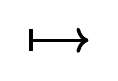
\begin{tikzpicture}
  \draw[|->, line width=1.25pt] (0,0) -- (0.75,0);
 \end{tikzpicture}}
 
%{
\includegraphics[scale=0.1]{single_arrow.png}}
%{
\includegraphics[scale=0.1]{double_arrow.png}}

\newcommand{\trstep}{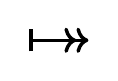
\begin{tikzpicture}
  \draw[|->>, line width=1.25pt] (0,0) -- (0.75,0);
 \end{tikzpicture}}
 
 
 
\newcommand{\ca}{\xrightarrow[]{ca}}

\newcommand{\caname}{\textit{convert-assignments}}

\mathchardef\mhyphen="2D


\makeatletter  % Allow the use of @ in command names
\long\def\@makecaption#1#2{%
  \vskip\abovecaptionskip
  \sbox\@tempboxa{{\captionfonts #1: #2}}%
  \ifdim \wd\@tempboxa >\hsize
    {\captionfonts #1: #2\par}
  \else
    \hbox to\hsize{\hfil\box\@tempboxa\hfil}%
  \fi
  \vskip\belowcaptionskip}
\makeatother   % Cancel the effect of \makeatletter
% ---------------------------------------

% Define Appendix refs
\crefname{app}{appendix}{appendices}
\Crefname{app}{Appendix}{Appendices}

% Add Figures folder to the graphics path
\graphicspath{{Figures/}{figures/}}

% Options for hyperref
\hypersetup{
    bookmarksnumbered=true,
    bookmarksopen=false,
    bookmarksopenlevel=0,
    colorlinks=false,
    pdfstartview=Fit,
    pdfborder={0 0 0},
}

\newcounter{qcounter}
\providecommand{\keywords}[1]{\textbf{\textit{Keywords:}} #1}


\begin{document}

% Declarations for Front Matter
\title{Verifying correctness of a Chez Scheme compiler pass}
\author{Ian Atol}
\degreemonth{June} \degreeyear{2021} \degree{Master of Science}
\defensemonth{June} \defenseyear{2021}
\numberofmembers{3}
   \chair{John Clements, Ph.D. \linebreak Professor of Computer Science}
   \othermemberA{Aaron Keen, Ph.D. \linebreak Professor of Computer Science}
   \othermemberB{Stephen R. Beard, Ph.D. \linebreak Assistant Professor of Computer Science}
\field{Computer Science} \campus{San Luis Obispo}
\copyrightyears{seven}


\maketitle
\begin{frontmatter}

% Custom made for Cal Poly (by Mark Barry, modified by Andrew Tsui).
\copyrightpage

% Custom made for Cal Poly (by Andrew Tsui).
\committeemembershippage

\begin{abstract}
We present a proof of correctness for a pass of the Chez Scheme compiler over a subset of the Scheme programming language. To improve trust in our proof approach, we provide two different validation frameworks. The first, created with the Coq proof assistant, is a partial mechanization of the proof, notably implementing a formal semantics for our subset of Scheme. This framework was designed to serve as a basis for the future work of a complete mechanization of our proof. The second framework uses an existing implementation of the Scheme semantics to demonstrate correctness of the pass on a variety of individual examples. We discuss our proof and frameworks in-depth, and give a historical background on compiler correctness proofs and their mechanization.
\end{abstract}

\begin{acknowledgements}
\noindent
Thanks to:
\begin{itemize}
    \item My friends and family for supporting me unconditionally, bringing me food on many occasions, and reminding me to step outside every now and then.
    \item John Clements for putting up with me borrowing books for way too long, for being contagiously excited about programming languages, and for believing in me.
    \item Aaron Keen for putting in extra effort to help me out several times, for teaching me Rust, and for introducing me to type theory.
    \item Zo\"e Wood for pointing me exactly in the right direction, and to exactly the right people.
\end{itemize}

\end{acknowledgements}

\tableofcontents

\listoftables

\listoffigures

% Add CHAPTER into table of contents.
\addtocontents{toc}{%
   \noindent CHAPTER
}

\end{frontmatter}

\pagestyle{plain}

\renewcommand{\baselinestretch}{1.66}

\chapter{Introduction}
As computers become increasingly ubiquitous in our lives, the software running on them becomes even more important, but also more complex. For example, we are lucky to live at a time where computers can help us to live longer by powering advanced medical equipment \cite{med_software}, but the grave consequences of errors in the software of these devices is clear \cite{sandler2010killed}. This simultaneously increasing complexity and importance is troubling, since these two concepts are traditionally at odds. 

To confront these issues, many researchers are hard at work with the goal of ensuring reliability of software. One approach to this problem, \textit{static analysis}, aims to prove properties of programs before they are run. For example, static analysis could be performed on a program to eliminate a certain type of error from it \cite{ayewah2008using}. One approach to static analysis uses the \textit{semantics} \cite{schmidt1996programming} of a language to devise formal proofs about the ``meaning'' of a program.

However, the journey from source code written by a human to the code that is actually executed by a computer is not trivial. For many languages, source code must be translated by a tool called a \textit{compiler} to machine code that the computer can run. If the compiler makes an error in translation, any proof about the behavior of that program is now forfeit. Essentially, any proof made about the source code of a program makes the assumption that a compiler will faithfully translate its meaning to the computer.

As our programs grow in size and complexity, so too do our compilers, adding additional features and optimizations. This means that our compilers themselves are caught in the same troubling convergence of increasing complexity and importance. One natural thought is to look to prove properties about the compilers themselves. Namely, we want to prove that our compilers translate correctly --- that the meaning of any program given to them is preserved in the process of translation. For example, the CompCert project \cite{leroy2019compcert} formally verifies the correctness of a compiler for a large subset of C. If we make proofs about programs in this subset, we can be sure that their claims are preserved through the compilation process. 

In this paper, we provide a proof of correctness for a single pass of the Chez Scheme compiler \cite{dybvig2011chez}, called \textit{np-}\caname. To support and validate our reasoning, we provide two different frameworks for producing evidence of our proof. The first is a formal model of the subset of the Scheme semantics that we use to reason about the compiler pass. Built using the Coq proof assistant \cite{barras_coq_1997}, this model provides a framework for using intuitionistic logic to prove properties about Scheme and Scheme programs with a high degree of trustworthiness. This model was meant to be the basis of a mechanization of our proof, but the full mechanization ended up being outside of the scope of this thesis. The second framework provides a way of testing individual programs for semantic preservation over the \caname\ transformation. This framework, created with the Racket \cite{felleisen2015racket} language, uses an existing implementation of the Scheme formal semantics to validate our proof technique on given example programs.

We hope that this work can serve as a trustworthy proof of the correctness of this compiler pass, and more generally hope to see a future where we can wholly trust that our compilers are translating critically important programs correctly.
\chapter{Background}
\section{Compiler Correctness}
``Can you trust your compiler?''

This quote begins the paper on the CompCert project \cite{leroy2019compcert}, one of the largest proofs of compiler correctness. These proofs aim to provide trust in our compilers by formally verifying that they preserve the meaning of programs that they translate. CompCert provides such a proof for a purpose-built compiler that translates a large subset of C to machine code. For large languages like C, which have correspondingly large compilers, these proofs are notoriously difficult --- CompCert totals around 100,000 lines of code in the Coq proof assistant, and took over 6 years to complete \cite{leroy_formal_2009}.

In this section, we will review some background on compiler correctness proofs. To do so, we have to look not only at the history of such proofs themselves, but also the evolution of tooling that embeds mathematical logic systems and allow for management of large-scale proofs. Without such systems, modern, large-scale projects such as CompCert would not be possible, so the advancement of these tools is key to understanding the progression of compiler correctness proofs. 

\subsection{History}
The first known formal proof of compiler correctness comes from John McCarthy and James Painter \cite{mccarthy_correctness_1967}. In their 1967 paper, they prove that a compiler that translates simple arithmetic expressions to machine code is correct. Despite the simplicity of the example source language, the paper is very important in that it sets up a methodology for computational proofs of compiler correctness. For example, their method of proof by structural induction of expressions is still an oft-used strategy for reasoning about properties of a languages programs.

McCarthy and Painter's proof was intentionally simple, so much so that it was able to be manually formulated and checked. However, when dealing with larger languages, case analysis of language expressions quickly generates too large of a proof to keep track of by hand. Because of this complexity, modern proofs of compiler correctness universally utilize programs called proof assistants that embed mathematical logic systems and can computationally verify the consistency of theorems defined within them. These assistants are necessary to aid with management of proofs at such a large scale. As such, their creation and development has been strongly connected to the progress of compiler correctness proofs.

\subsubsection{Proof Checkers, Intuitionistic Logic, and Mechanized Proofs}\label{sxn:mech_background}
The first large-scale attempt to \textit{mechanize} mathematics, or formally define mathematics in a way tractable by a computer, was Nicolaas Govert de Bruijn's Automath language \cite{nederpelt_survey_1994}. Automath was an early example of a correspondence between logic and programs --- in the Automath language, theorems are defined as types, and proofs consist of showing that these types are inhabited by some value. This means that the definitions and proofs of theorems within Automath's logical framework are represented as a computer program. This relationship between programs and logic is also at the core of the Curry-Howard correspondence between deductive logic and the simply-typed Lambda Calculus.

Research into these sorts of program-logic relations continued into the 70s and 80s, with the development of the \textit{Intuitionistic Theory of Types} \cite{martin-lof_intuitionistic_1998} by Per Martin-Löf and the polymorphic Lambda calculus \cite{girard_interpretation_1972} by Girard. These theories also rely on the Curry-Howard correspondence to tie their dependently typed programs to statements in \textit{intuitionistic logic}. 

Intuitionistic logic is a kind of logical system that requires \textit{evidence} or \textit{witnesses} of a statement to prove its validity. That is, to prove that a statement $A \xrightarrow{} B$ is true in an intuitionistic logic, one must use the axioms of the logic to \textit{construct} evidence that B is true from the existing evidence that A is true. One important property of these intuitionistic logics that follows their constructive foundation is that the law of the excluded middle is not true in these systems --- that is, we cannot perform indirect proofs, for example by contradiction. In other words, proving that $\lnot A$ is not true does not suffice as proof of A. In this way, intuitionistic logic requires more direct proof of statements. In systems such as Automath, where a correspondence between logical statements and programs is established, a constructive proof of a statement corresponds to an algorithm that generates the program representing that statement. Because of this strong correspondence, these constructive, intuitionistic proofs lend themselves extremely well to automation, just as developers may automate complex parts of a software project.

A further example of the natural connection between intuitionistic logic and dependent type theory is Thierry Coquand's Calculus of Inductive Constructions\cite{coquand_calculus_1986, paulin-mohring_introduction_2015}. This system combines Intuitionistic Type Theory and the polymorphic Lambda Calculus into a single calculus that also provides support for writing specifications that automatically come equipped with powerful induction principles.

While the Calculus of Inductive Constructions is powerful, it is unwieldy and hard to manually construct large programs with. For this reason, the Coq proof assistant \cite{barras_coq_1997} was devised. An extension of the original Automath language, Coq embeds the Calculus of Inductive Constructions, and also provides a high level tactics language \cite{delahaye_tactic_2000} on top of the core calculus. This tactics language provides automation in the form of syntactic sugar and algorithmic search of core calculus expressions to assist in the construction of large proof terms. This tactics language greatly increase the size of proofs that Coq can handle --- indeed, Coq programmers spend the majority of their time writing, configuring, and refactoring proofs using the tactics language, so at a much higher level than using the calculus itself. 

Because of its support for automation, its history, and a large amount of libraries and community support, Coq is a natural choice for large-scale mechanized proofs. One example of this is the proof of the four color theorem. This theorem was famously unsolved until Coq's automation features made its extensive case analysis proof feasible \cite{gonthier_formal_2008}. Other projects realized in Coq include the Univalent Foundations project \cite{voevodsky_univalent_2010}, which attempts to build a foundation for mathematics based on a type theory, and the CompCert project.

Finally, while we focus on Coq because of its usage in this project, a plethora of modern proof assistants exist \cite{geuvers2009proof, barendregt2001proof}. Some examples of modern languages that are used as proof assistants include Lean \cite{de2015lean}, Agda \cite{bove2009brief}, and Idris \cite{brady2013idris}. More and more frequently, and in various fields, these tools are used to provide mechanized proofs to accompany research papers. In the next section, we will review some modern compiler correctness projects, all of which use proof assistants to validate their approach.

\subsubsection{Verified Compiler Projects}\label{sxn:new_proofs}
Table \ref{tab:cc_projs} gives an overview of some compiler verification projects.
\begin{table}[]
    \centering
    \begin{tabularx}{\textwidth}{l|X}
         CompCert \cite{leroy2019compcert} & A verified compiler from C to various assembly languages, written and proven in Coq. \\
         CakeML \cite{kumar2014cakeml} & A verified compiler for a subset of ML, verified using Isabelle/HOL \cite{nipkow2002isabelle} \\
         CertiCoq \cite{anand2017certicoq} & A verified Coq compiler, also written and proven using Coq \\
         VLISP \cite{guttman_vlisp_1995} & A verified (but not mechanized) compiler for an early version of Scheme \\
         ClightTSO \cite{sevvcik2011relaxed} & An extension of CompCert that verifies a compiler for a C-like language that supports shared-memory concurrency. \\
         Concurrent Java \cite{lochbihler2010verifying} & A verified compiler for a subset of Java that supports threading, formalized in Isabelle/HOL.
    \end{tabularx}
    \caption{Sampling of verified compiler projects}
    \label{tab:cc_projs}
\end{table}

So concludes our background on compiler verification projects and history. In the next section, we will review the Scheme language and its compiler, as background for our later proof of correctness of one of its passes.

\section{Scheme}
Scheme is a functional language based on LISP. While LISP supported functional programming (i.e. first-class functions and recursion) with a "lambda" notation \cite{mccarthy1960recursive}, Scheme was the first LISP to closely mirror the call-by-value Lambda Calculus by utilizing static scoping for its variable bindings. In addition, as Scheme evolved and added more features, its macro system, syntactic pattern matching, and homoiconity made it a language suited to modelling other programming languages. Because of this, Scheme has seen extensive use in the area of programming languages research. 

In this section, we will give some historical background on Scheme, then review the version of Scheme we chose for this project, and finally touch on the Chez Scheme compiler itself.
\subsection{Lambda Calculus, LISP, and Scheme}
The Lambda Calculus is a model which Alonzo Church and his students developed in the late 1930s \cite{church1936unsolvable} as a way to categorize a certain kind of number problem. It was later famously shown to be equivalent to Turing Machines, and together define the standard class of known computable problems \cite{sep-church-turing}. While programming languages are inherently based in computation, the Lambda Calculus was later found to be capable of simply and accurately modeling the behavior of parts of ALGOL 60 \cite{landin1965correspondence}, a programming language based on procedures.

While working on a LISP-based language for modeling actor-based concurrency \cite{sussman_first_1998}, Steele and Sussman discovered that their new language had a strong, unexpected connection with the Lambda Calculus. While LISP supported lambda notation for functions, it did not handle variable naming or scoping in the same way as Church's original model. However, as Steele and Sussman shaped their version of LISP, they found that they were able to greatly simplify the language by following the semantics of the call-by-value version of the Lambda Calculus closely. The resulting language, called Scheme, was shown to be able to effectively model a wide variety of other programming languages, while still maintaining a small size and a tidy semantics \cite{steele1978revised}. 

Because of its small size and close connection to both the well-studied Lambda Calculus and popular LISP language, Scheme saw widespread usage for research in the area of programming languages. Using Scheme's powerful pattern matching and tools for syntactic abstraction, researchers can quickly create a model of their work to accompany a more detailed paper. We use Scheme in a similar manner for our own work in this paper (see section \ref{sxn:rkt}).

Scheme has a language standard in the form of the Revised$^n$ Report on the Algorithmic Language Scheme (R\textit{n}RS). This standard defines a formal syntax and semantics for a large subset of Scheme, while leaving some areas up to the specific implementation. Our work is based on one of the more recent standards for Scheme --- R6RS \cite{sperber_revised6_2009}.

\subsection{Scheme Verification}
Along with its widespread usage in programming languages research, Scheme has itself been the target of formal verification projects. One such project, VLISP \cite{guttman_vlisp_1995}, was based on an earlier, denotational semantics for Scheme \cite{IEEE_scheme}. The initial VLISP project led to several formally verified extensions as well as explorations into representing Scheme using an operational semantics \cite{guttman_vlisp_system_1995}.

\subsection{The Chez Scheme compiler}
The Chez Scheme compiler is an optimizing compiler written in Scheme itself. It provides an implementation of Chez Scheme \cite{dybvig1983chez}, which follows the R6RS standard and adds some additional features. Notably, it is the compiler for many Scheme dialects, including the Racket language \cite{felleisen2015racket}. It notably utilizes the Nanopass framework \cite{keep2013nanopass} at its foundation. The framework provides a domain specific language embedded in Scheme, designed for quickly defining languages and translations between them. An example of a Nanopass language definition from the Chez Scheme compiler is shown in figure \ref{fig:nanopass_ex}. This example shows an intermediate language (L4) that removes set! expressions from another language that it extends (L3). We will see later that this definition corresponds to the pass that we prove correctness of (see section \ref{sxn:ca-pass}).

\begin{figure}
    \centering
    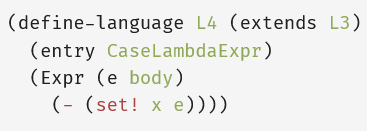
\includegraphics[scale=0.75, keepaspectratio]{figures/np_def.png}
    \caption{Example of a language definition in Nanopass}
    \label{fig:nanopass_ex}
\end{figure}

In this project, we build a framework for reasoning about Scheme and use it to prove correctness of one pass of the Chez Scheme compiler. One reason we chose to target the Chez Scheme compiler for verification was because of its usage of the Nanopass framework. Since passes are distinctly separated and small in size by design, correctness proofs of individual passes should be simpler, and also are able to be easily composed to larger proofs about correctness of a sequence of passes.

\chapter{Formalizing Scheme}
Any proof about properties of Scheme, such as a proof about semantic preservation over a transformation, needs to be based on a formal definition of the language. Therefore, our first step in writing such a proof is to formally define the Scheme language. For the sake of simplifying the proof, we excluded many features --- in general, these are features where our transformation doesn't change very much, but are complex enough to add substantial difficulty to our proof. These excluded features are discussed in more detail in section \ref{excluded}.
\section{R6RS Scheme}
Fortunately, Scheme is already well-defined. The R6RS language standard \cite{x} provides a formal specification of Scheme's syntax and semantics, and also gives an implementation of the semantic model in the PLT Redex language. As previously mentioned, we excluded many features from this formal definition for ease of reasoning. Below is our modified version of R6RS Scheme

\subsection{Syntax}
Figure \ref{fig:syntax} shows an EBNF representation of the syntax for our subset of Scheme.
\newpage
\begin{figure}[h]
    \centering
\begin{bnfgrammar}
    P ::=
        (store (sf ...) e)
    ;;
    sf ::=
        (x v)
    |   (pp (cons v v))
    ;;
    e ::=
        nonproc
    |   proc
    |   (begin e e ...)
    |   (if e e e)
    |   (e e ...)
    |   (set! x e)
    |   (values v)
    |   x
    ;;
    v ::=
        nonproc
    |   proc
    ;;
    nonproc ::=
        pp
    |   null
    |   n
    ;;
    proc ::=
        (lambda (x) e)
    |   (lambda () e)
    |   car
    |   cdr
    |   cons
    |   set-car!
    |   set-cdr!
    |   +   
    |   -
    |   /
    |   *
    ;;
    pp ::=
        [pair pointers]
    ;;
    x ::=
        [variables]
    ;;
    n ::=
        [integers]
\end{bnfgrammar}
\caption{The syntax for our subset of Scheme}
    \label{fig:syntax}
\end{figure}

Variables and pair pointer names are restricted to exclude keywords.

\subsubsection{Evaluation Contexts}
While we have presented a syntax for programs in our language, as we will see in the next section, our semantics operates on programs decomposed into an \textit{evaluation context} and a reducible expression.

Evaluation contexts utilize a syntax of \textit{holes} and \textit{contexts} to isolate certain sub-expressions in order to apply semantic rules on them.

For example, we can decompose the following program to allow for evaluation of the expression in the \textit{$e_1$} position of the if expression.

$(store\ (sf\ \dots)\ (if\ ((lambda\ (x)\ \#t)\ 5)\ \#t\ \#f)) = C[((lambda\ (x)\ \#t)\ 5)]$ where $C = (store\ (sf\ \dots)\ (if\ [\ ]\ \#t\ \#f)$.

The key feature of evaluation contexts is that they can control where evaluation occurs. These contexts cleverly enforce a canonical order of evaluation, which means that any expression that is reducible has only one possible step to take. We prove this property of our evaluation contexts in section \ref{sxn:det_sem}.

Since we have removed many features, we use only the evaluation contexts relevant to expressions that are still in our language:

\begin{figure}[h]
    \centering
\begin{bnfgrammar}
    C ::= (store (sf ...) $F^{*}$)
    ;;
    F ::= [ ]
    |   (v ... $F^{\circ}$ v ...)
    |   (if $F^{\circ}$ e e)
    |   (set! x $F^{\circ}$)
    |   (begin $F^{*}$ e e ...)
    ;;
    $F^{*}$ ::= [ ]$^{*}$
    |   F
    ;;
    $F^{\circ}$ ::= [ ]$^{\circ}$
    |   F
\end{bnfgrammar}
    \caption{The evaluation contexts for our subset of Scheme}
    \label{fig:eval_ctx}
\end{figure}

Here, $F^{*}$ and $F^{\circ}$ refer to contexts that perform promotion or demotion between single values and (values v) expressions. The relevant semantics rules are presented in figure \ref{fig:Sem2}. Though we do not support multiple values, we wanted to preserve this feature of the formal semantics to increase extensibility of our subset. That way, our proofs will be more easily adaptable if the language is modified to include multiple values.

\subsection{Semantics}
Figures \ref{fig:Sem1} and \ref{fig:Sem2} show the operational semantics for our subset of Scheme.
\begin{figure}
\centering
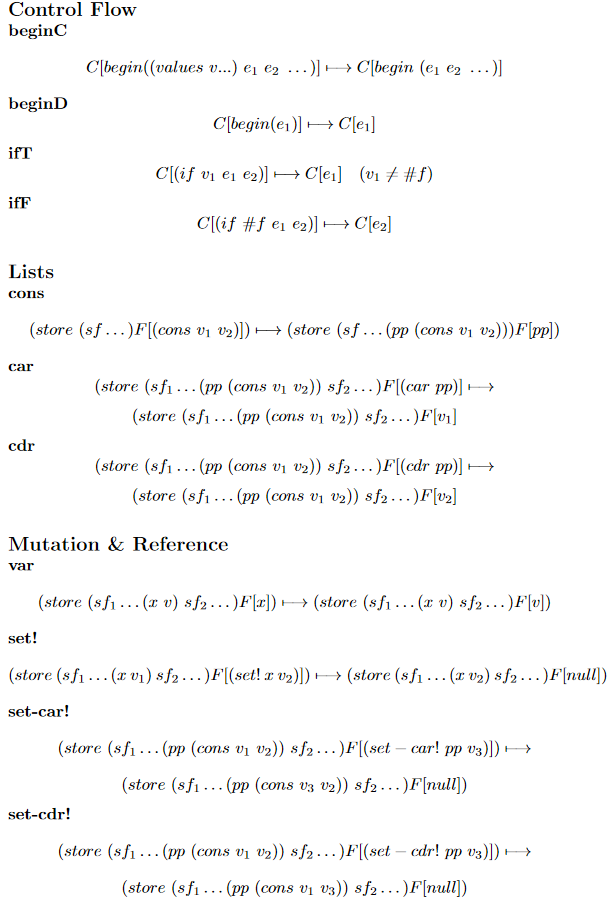
\includegraphics[width=\textwidth,height=\textheight,keepaspectratio]{figures/sem_1.png}
    \caption{Control flow, list, and mutation semantics for our subset of Scheme}
    \label{fig:Sem1}
\end{figure}

\begin{figure}
\centering
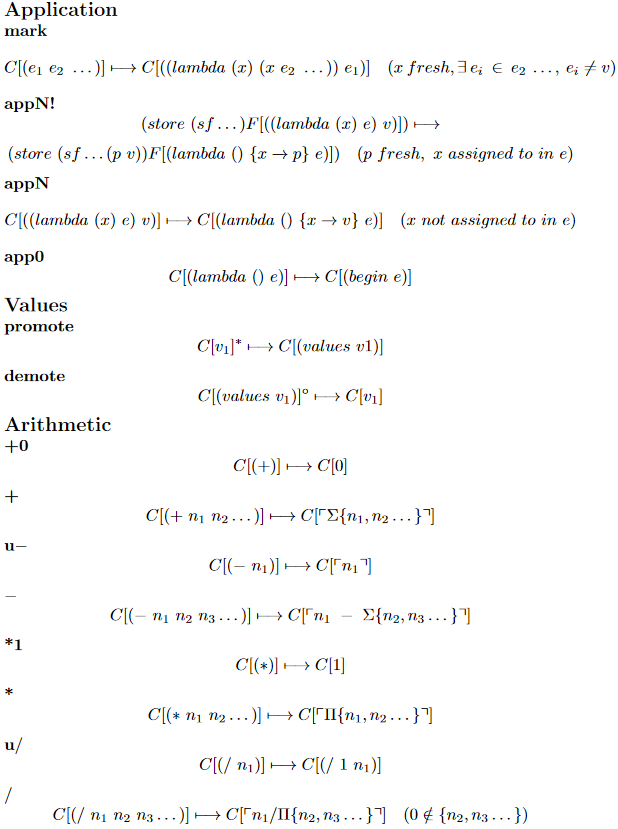
\includegraphics[width=\textwidth,height=\textheight,keepaspectratio]{figures/sem_2.png}
    \caption{Application, value handling, and arithmetic semantics for our subset of Scheme}
    \label{fig:Sem2}
\end{figure}

We define x being "assigned to" as x being the target of a set!

Some discussion of our semantic rules and how they work together to evaluate Scheme programs is required.

\subsubsection{Control Flow}\label{sxn:sem_cf}
\textbf{beginC} works by removing values from the front of a $(begin\ \dots)$ expression. Together with the begin evalaution context, \textbf{beginC} evaluates and removes each sub-expression in a $(begin\ \dots)$ expression until it has only a single sub-expression remaining. Then, the \textbf{beginD} rule applies to consider that expression alone. This is how the requirement that Scheme begin expressions return the value of the last sub-expression is enforced.

\textbf{ifT} and \textbf{ifF} behave as expected, with the minor quirk that any value that is not $\#f$ is considered true.

\subsubsection{Lists}\label{sxn:sem_lists}
\textbf{cons}, \textbf{car}, and \textbf{cdr} handle pairs (and therefore lists) in our language. Notably, \textbf{cons} places pairs into the store and returns a pointer to the store location in return. \textbf{car} and \textbf{cdr} therefore take a pair pointer as their argument to access the first and second values of the pair respectively.

\subsubsection{Mutation \& Reference}\label{sxn:sem_assign}
\textbf{var}, \textbf{set!}, \textbf{set-car!}, and \textbf{set-cdr!} handle assignment in the language. \textbf{var} is a fairly straightforward step that takes a variable referring to a store location and returns the value at that location. The assignment functions replace values in a store location in a similar way. One thing to note is that \textbf{set!} requires that its variable argument already exists in the store. As we are not considering top-level variables (see section \ref{sxn:excluded}), \textbf{set!} can only modify existing store locations created during lambda application.

\subsubsection{Application}\label{sxn:sem_app}
\textbf{mark} isolates un-evaluated sub-expressions in chained applications. Note that \textbf{mark} enforces a left to right evaluation order.

\textbf{appN!} is the application semantic rule for lambda expressions that contain assignment in their bodies. Since naive assignment into such lambda expressions would result in erroneous expressions like (set! 4 5), \textbf{appN!} first creates a fresh store location containing the value to be substituted and then performs substitution with a pointer to that location rather than with the value itself. Then, assignments inside the lambda expression's body can properly evaluate. The \textbf{appN} rule applies naive substitution in lambda expressions that do not contain assignment. As we will see in section \ref{sxn:ca-pass}, excluding these non-assigned variables from the store is integral to our proof of correctness of the compiler pass we are considering.

\subsubsection{Values \& Arithmetic}\label{sxn:sem_vals_math}
Finally the \textbf{promote} and \textbf{demote} rules deal with wrapping values to satisfy the requirements of their evaluation contexts. While this feature is vestigial in our semantics, we include it for purposes of extensibility.

The following rules present a fairly typical system for performing integer arithmetic. Note the side conditions for ensuring no division by zero takes place.

\subsubsection{Excluded Features\label{sxn:excluded}}
In the interest of shortening a potentially extensive proof, we chose to remove many features from the formal R6RS semantics. Additionally, some features of Scheme were not originally included in the formal R6RS semantics, likely due to complexity of formalization.

The features we chose to exclude were: quote, multiple argument lambda expressions (and generally multiple values as arguments), exceptions, equivalence testing, call/cc and dynamic wind, and letrec. I/O, the macro system, and the numerical tower were originally excluded from the R6RS semantics. While this list certainly contains major features of Scheme, we believe we have captured enough of the language to accurately represent and prove correctness of our transformation.

Another quirk of the formal R6RS semantics is that evaluation order of expressions is left up to the implementation. However, this means that without modification, the semantics are non-deterministic --- application of their version of the \textbf{mark} rule results in a set of steps each representing a different choice of evaluation order. In our semantics, we modify \textbf{mark} to follow a left-to-right evaluation order. This simplification allows us to prove semantic determinism, which we use in our proof. While our transformation shouldn't be affected by a different evaluation order, it is theoretically possible that an implementation of Scheme could enforce an evaluation order that would invalidate our results. We cover this in more detail in section \ref{sxn:eval_order}.

Finally, while set! expressions that mutate top-level variables are present in Scheme, these top-level set! expressions are converted to "set-top-level!" expressions in a pass prior to the one we are considering. Therefore, we can assume that all set! terms we encounter refer to variables in their local scope. Further, handling top-level variables in general turned out to be a major difficulty in modeling this pass. Since top-level variables are not affected by this pass, we are not including them in our subset. Therefore, we do not include letrec, as this is how top-level variables are implemented by the semantics.

\chapter{Proving correctness of \textit{np-convert-assignments}}\label{chap:proof}
While the entire Chez Scheme compiler translates Scheme to machine code, the \caname\ pass performs a single intermediate step in this process by performing a Scheme-to-Scheme transformation on some expressions. As its name suggests, the purpose of the \caname\ pass is to \textit{convert} variable \textit{assignment} expressions to a different form. Since both the source and target languages are Scheme, we can reason about the pass solely using Scheme's formal \textit{operational semantics}, a rigorously defined standard for reducing Scheme expressions.

We will first review the pass itself and the transformation that it performs. Then, we will define our notion of semantic preservation, and use some properties of the semantics as well as some relations defined atop it to show that the transformation does indeed preserve the semantics of a program.
\section{The \textit{np-convert-assignments} pass\label{sxn:ca-pass}}
\subsection{Assumptions}
One important note about \caname\ is that it uses special, decorated expressions in both its source and target languages. Since we do not have have a formal framework for asserting the meaning of these decorated Chez Scheme expressions, we make the critical assumption that they abide to the relevant rules of the R6RS formal semantics. From observation, this assumption seems to hold true, as the decorated expressions can be consistently \textit{erased} down to normal Scheme expressions (see Figure \ref{fig:chez_erase} for an example of a term in the source language of \caname\ compared to its \textit{erased} version in the language defined by the formal semantics).

\begin{figure}[h]
    \centering
    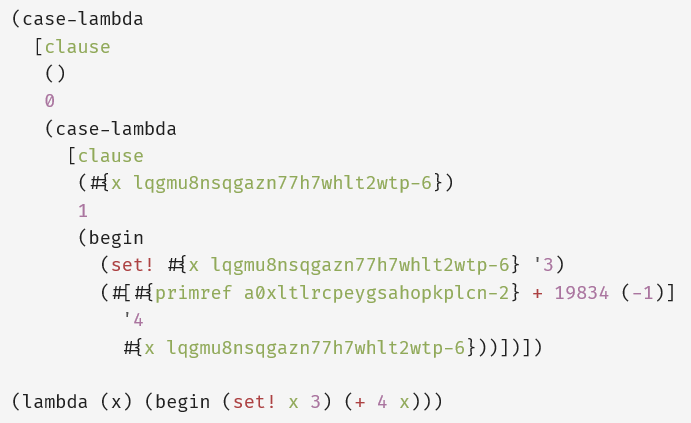
\includegraphics[scale=0.75, keepaspectratio]{figures/chez_erase.png}
    \caption{Example of \textit{erasing} Chez Scheme term decoration.}
    \label{fig:chez_erase}
\end{figure}

Another area where we must make an assumption is in developing a model of \caname\ to reason about. The code for actually executing the pass contains and operates on expressions that are not covered by the R6RS semantic model. Therefore, we attempt to faithfully recreate the effects of the transformation on the expressions in subset of the formal semantics that we are considering. Our analogous \caname\ function was created through careful examination of the source code and observation of input and output of the pass for various examples.

\subsection{Intuition}
The \textit{np-convert-assignments} pass removes indefinite-extent assignments and replaces them with assignments that have a defined scope. This pass is quite small, defined in about 40 lines in the production Chez Scheme compiler. The size of our proof and accompanying frameworks relative to the size of the transformation is a testament to the difficulty of verifying compilation correctness.

The intuition for the pass is best acquired through observing an example of a transformation on a small program:

\begin{figure}[h]

$ca_{prog}$(store ((x $v_1$)) (lambda (y)

\qquad \qquad \ \qquad \ \qquad \quad \ (begin 

\qquad \qquad \ \qquad \ \qquad \qquad \ (set! y $v_2$) 

\qquad \qquad \ \qquad \ \qquad \qquad \ (+ x y)))) =
 
\qquad \ (store (($pp_x$ (cons $\hat{v_1}$ null))) (lambda (t)

\qquad \qquad \qquad \qquad \qquad \qquad \qquad \quad \ ((lambda (y) 

\qquad \qquad \qquad \qquad \qquad \qquad \qquad \qquad \ (begin 

\qquad \qquad \qquad \qquad \qquad \qquad \qquad \qquad \quad \ (set-car! y $\hat{v_2}$) 

\qquad \qquad \qquad \qquad \qquad \qquad \qquad \qquad \quad \  (+ (car $pp_x$) (car y)))) 

\qquad \qquad \qquad \qquad \qquad \qquad \qquad \quad \ \ (cons t null))))

Where $\hat{a}$ means the appropriate \caname\ function applied to a.
    \caption{Motivating example for the \caname \ pass.}
    \label{fig:ca_example}
\end{figure}

We can immediately see the primary action of the pass --- to remove set! expressions. We can see that the set! expression inside the begin expression is transformed to a set-car! expression. Notice also the recursive call on the value of the set! expression. Depending on if a variable is in the store or enclosed in a lambda, we may transform it into a pointer or not, as shown by the transformation that occurs to the variables x and y respectively.

We can also see how lambda expressions are modified to support the transformation of set! expressions. Since its arguments are now assumed to be cons cells, we have to first wrap its arguments inside of a list. This is also the reason we do not change $y$ to $pp_y$, as at this point it is still an argument to the lambda expression.

Finally, we can see how $ca$ deals with store locations of partially evaluated programs. Since the \textbf{appN!} rule is the only one that can create new non-list store locations, we can assume that variables in the store correspond to previously evaluated lambda abstractions. Therefore, we must treat variables and set! expressions that refer to store locations as transformation targets. We also retroactively convert these previously evaluated store locations. In this case, we do change $x$ to $pp_x$, so that expressions that contain it can properly evaluate.

% Some explanation for these examples is required. The first example is one of the simplest --- it transforms a variable reference to a call to \textit{car} on a pair pointer representing that variable. We will see in the next examples why this pair pointer conversion is necessary, but we can see clearly the transformation that occurs to variable references. It is also important to note a slight abuse of our notation in this example: that we perform transformation on an evaluation context ($\hat{P}$). While the pass does not actually operate on decomposed programs, we use this notation for clarity and to be able to isolate transformations on specific parts of a program. In section \ref{sxn:ctx_trans}, we show that this way of transforming a program that is decomposed into a context and an expression is the same as transforming the program before decomposition.

% The second example shows the main purpose of the transformation --- to remove indefinite extent set! expressions from the language and replace them with set-car!. One important note about $x$ in this example is that it is always referring to a bound variable, though the lambda expression that bound it may have already been evaluated, as we consider in example 4. In that case, we know the variable was bound because it will be present in the store. Because we are not allowing top-level variables in our subset of the semantics, we can make this assumption and transform all set! that we encounter.

% The third example demonstrates the transformation of a lambda expression that contains an assigning set! expression. The original lambda expression is wrapped in an additional lambda expression and applied to the argument of that lambda expression wrapped in a cons cell. We can also see the transformation of the assigning set! expression. The purpose of this specific transformation is to make sure that all of the set! calls and variable references inside the lambda expression still work. Since they have been transformed to operate on lists, this step of the transformation ensures that they will always receive a list as their argument.

% The fourth example exhibits the behavior of the transformation on a partially evaluated program. Since the \textbf{appN!} semantic rule is the only rule that adds variables to the store, we can assume that if a variable is in the store, it was the target of a set! somewhere in the body of the lambda that was evaluated using \textbf{appN!} (since this is a side condition of the rule). Therefore, for the transformation to work correctly on partially evaluated programs, we need to transform each variable in the store that is not already a pair pointer. Note that all variables transformed this way are converted to pair pointers, since they now refer to cons cells. Therefore, after a transformation, our store will contain only pair pointers.
\subsection{Definition}
Figure \ref{fig:ca_fxs} defines our model of the transformation as functions on the syntax of our language. For notational brevity, we assume that each function has access to the store and a list of all names that are the target of a set! in the program.
\begin{figure}
    \centering
\begin{definition} {\large\textbf{ca$_{prog}$}} --- Programs

$ca_{prog}((store\ (sf \dots)\ e)) = (store\ (ca_{sf}(sf) \dots)\ ca_e(e)) $

\end{definition}

\begin{definition} {\large\textbf{ca$_{sf}$}} --- Store Locations

$ca_{sf}((x\ v)) = (pp_x\ (cons\ ca_e(v)\ null))$

$ca_{sf}((pp\ (cons\ v_1\ v_2))) = (pp\ (cons\ ca_e(v_1)\ ca_e(v_2))$
\end{definition}

\begin{definition} {\large\textbf{ca$_e$}} --- Expressions

$ca_e((set!\ x\ e)) = (set \mhyphen car!\ pp_x\ ca_e(e))$

\qquad where x is in the store.

$ca_e((set!\ x\ e)) = (set \mhyphen car!\ x\ ca_e(e))$

\qquad where x is not in the store.

$ca_e(x) = (car\ pp_x)$

\qquad where x is in the store.

$ca_e(x) = (car\ x)$

\qquad where x is not in the store, but is assigned to somewhere in the program.

$ca_e(x) = x$

\qquad where x is not in the store or assigned to.

$ca_e((lambda\ (x)\ e)) = (lambda\ (t)\ ((lambda\ (x)\ ca_e(e))\ (cons\ t\ null)))$

\qquad where x is assigned to, t is fresh.

$ca_e((lambda\ (x)\ e)) = (lambda\ (x)\ ca_e(e))$ 

\qquad where x is not assigned to.

$ca_e((begin\ e_1\ e_2\ \dots)) = (begin\ ca_e(e_1)\ ca_e(e_2)\ \dots)$

$ca_e((e_1\ e_2\ \dots)) = (ca_e(e_1)\ ca_e(e_2)\ \dots)$

$ca_e((if\ e_1\ e_2\ e_3)) = (if\ ca_e(e_1)\ ca_e(e_2)\ ca_e(e_3))$

$ca_e((values\ v)) = (values\ ca_e(v))$

All other expressions are unchanged by $ca_e$.

\end{definition}

Finally, we define $ca_{ctx}$ for use in applying the pass to decomposed programs.

\begin{definition} {\large\textbf{ca$_{ctx}$}} --- Evaluation Contexts

$ca_{ctx}((store\ (sf\ \dots)\ F_{*})) = (store\ (ca_{sf}(sf)\ \dots)\ ca_{ctx}(F_{*}))$

$ca_{ctx}((v_1\ \dots\ F_{\circ}\ v_2\ \dots)) = (ca_e(v_1)\ \dots\ ca_{ctx}(F_{\circ})\ ca_e(v_2)\ \dots)$

$ca_{ctx}((if\ F_{\circ}\ e_1\ e_2)) = (if\ ca_{ctx}(F_{\circ})\ ca_e(e_1)\ ca_e(e_2))$

$ca_{ctx}((set!\ x\ F_{\circ})) = (set \mhyphen car!\ pp_x\ ca_{ctx}(F_{\circ}))$

\qquad where x is in the store.

$ca_{ctx}((set!\ x\ F_{\circ})) = (set \mhyphen car!\ x\ ca_{ctx}(F_{\circ}))$

\qquad where x is not in the store.

$ca_{ctx}((begin\ F_{*}\ e_1\ e_2\ \dots)) = (begin\ ca_{ctx}(F_{*})\ ca_e(e_1)\ ca_e(e_2)\ \dots)$

$ca_{ctx}([\ ]) = [\ ]$

$ca_{ctx}([\ ]_{*}) = [\ ]_{*}$

$ca_{ctx}([\ ]_{\circ}) = [\ ]_{\circ}$

\end{definition}
    \caption{\caname\ functions}
    \label{fig:ca_fxs}
\end{figure}
\newpage

\subsection{Lemmas}
Here we prove some properties of the \caname\ functions that are necessary for our later proofs.

\begin{lemma}\label{lem:trans_val} Transformation Preserves Values

If v is a value, then $ca_e(v)$ is a value.
\end{lemma}
\begin{proof}
By induction on the structure of our value expressions.

For most values, $ca_e$ makes no changes. For these cases, $ca_e(v)$ is trivially a value.

The only value expression which is modified by $ca_e$ is $(lambda\ (x)\ e)$, where x is the target of a set! inside of e. We can observe the transformation:

$ca_e((lambda\ (x)\ e)) = (lambda\ (t)\ ((lambda\ (x)\ ca_e(e))\ (cons\ t\ null)))$

We can clearly see that this is still a value, since it is of the form $(lambda\ (t)\ e')$, where $e' = ((lambda\ (x)\ ca_e(e))(cons\ t\ null))$

Therefore, we have shown that $ca_e$ preserves the value status of values that it transforms.
\end{proof}

\begin{lemma}\label{lem:trans_expr} Transformation Preserves Expressions

If e is a non-value expression, then $ca_e(e)$ is a non-value expression.
\end{lemma}
\begin{proof}
The non-value expressions that get transformed by $ca_e$ are:

\begin{enumerate}
    \item $x$
    \item $(set!\ x\ v)$
\end{enumerate}

$ca_e(x)$ evaluates to either $(car\ x)$, $(car\ pp_x)$, or just $x$, all of which are still expressions.

$(set!\ x\ v)$ similarly evaluates to either $(set \mhyphen car!\ x\ \hat{v})$ or $(set \mhyphen car!\ pp_x\ \hat{v})$, which are both still expressions.

Therefore, if $e$ is a non-value expression, $ca_e(e)$ will always be a non-value expression.

\end{proof}

\begin{lemma}\label{lem:trans_decomp} Transformation Preserves Decomposition

$ca_{prog}(C[e]) = ca_{ctx}(C)[ca_e(e)]$

for all evaluation contexts C and expressions p.

\end{lemma}
\begin{proof} We proceed by induction on the structure of our evaluation contexts.

Consider the cases of C: $(store (sf ...) F_{*})$

and the cases of $F_{*}$: $[\ ]_{*}$, $F$.

If $F_{*}$ is a hole, then we must show that 

$ca_{prog}((store (sf ...)\ e)) = ca_{ctx}((store (sf ...) [(ca_{e}(e))]))$

which follows from the definitions of $ca_{prog}$ and $ca_{ctx}$.

Otherwise, consider the cases of F: $[\ ]$, $(v \dots F_{\circ}\ v \dots)$, $(if\ F_{\circ}\ e\ e)$, $(set!\ x\ F_{\circ})$, and $(begin\ F_{*}\ e\ e \dots)$.

$[\ ]$ follows by definitions as before. 

In the case of  $(v \dots F_{\circ}\ v \dots)$, $(if\ F_{\circ}\ e\ e)$, $(begin\ F_{*}\ e\ e \dots)$, $ca_{ctx}$ makes no structural changes to the context other than the expected calls to $ca_{ctx}$ and $ca_e$ on sub-expressions. Therefore, it follows from our induction principle and the definitions of $ca_{ctx}$, $ca_e$ that the transformation preserves decomposition in these cases.

The interesting case, $(set!\ x\ F_{\circ})$, has a transformation occur in the evaluation context. There are two possibilities for the transformation of $(set!\ x\ F_{\circ})$:

\begin{enumerate}
    \item $ca_{ctx}((set!\ x\ F_{\circ})) = (set \mhyphen car!\ pp_x\ ca_{ctx}(F_{\circ}))$ if x is in the enclosing store.
    \item $ca_{ctx}((set!\ x\ F_{\circ})) = (set \mhyphen car!\ x\ ca_{ctx}(F_{\circ}))$ if x is not in the store (i.e. if x is bound by a lambda expression in some enclosing context).
\end{enumerate}

In case 1, we need to show that:

$ca_{prog}((store\ (sf \dots)\ (set!\ x\ F_{\circ}[p]))) = ca_{ctx}((store\ (sf \dots)\ (set!\ x\ ca_{ctx}(F_{\circ})[ca_e(p)])))$

Since we know x must be in the store, 

$ca_{prog}((store\ (sf \dots)\ (set!\ x\ F_{\circ}[p]))) = (store\ (ca_{sf}(sf) \dots)\ (set \mhyphen car!\ pp_x\ ca_{e}(F_{\circ}[p])))$. 

This case follows by definition of $ca_{e}$ and $ca_{ctx}$, and by our induction principle.

Case 2 follows similarly, except that x is not in the store, so 

$ca_{prog}((store\ (sf \dots)\ (set!\ x\ F_{\circ}[p]))) = (store\ (ca_{sf}(sf) \dots)\ (set \mhyphen car!\ x\ ca_{e}(F_{\circ}[p])))$. 

Therefore, we have shown that our transformation preserves decomposition for all cases.
\end{proof}








\newpage
\section{Proof Overview}
To prove that $ca_{prog}$ preserves the semantics of programs that it transforms, we must consider what we mean by semantic preservation. Since $ca_{prog}$ entirely removes an expression, set!, we cannot expect the transformed program to take \textit{exactly} the same steps. It seems reasonable, then, to say that a program's semantics are preserved over a transformation if the transformed program takes \textit{equivalent} steps. 

To formalize this informal definition, we must first define a way for a program to take multiple steps:
\begin{definition}
Transitive, reflexive closure of $\step$
\begin{enumerate}
    \item $a$ \trstep\ $c$ if $a$ \trstep\ $b$ and $b$ \trstep\ $c$ (Transitivity)
    \item $a$ \trstep\ $a$ (Reflexivity)
    \item $a$ \trstep\ $b$ if $a\ \step\ b$ (Closure)
\end{enumerate}
\end{definition}

The intuition for the reflexive, transitive closure of $\step$ is that it relates expressions that have zero or more single steps between them.

Our definition of step \textit{equivalence} uses the idea of simulation. That is, if a relation is a simulation relation, then related programs take equivalent semantic steps. The intuition for such a relation is shown by Figure \ref{fig:sim_diagram}. We formally define our notion of a simulation relation in section \ref{sxn:sim}.

\begin{figure}
    \centering
    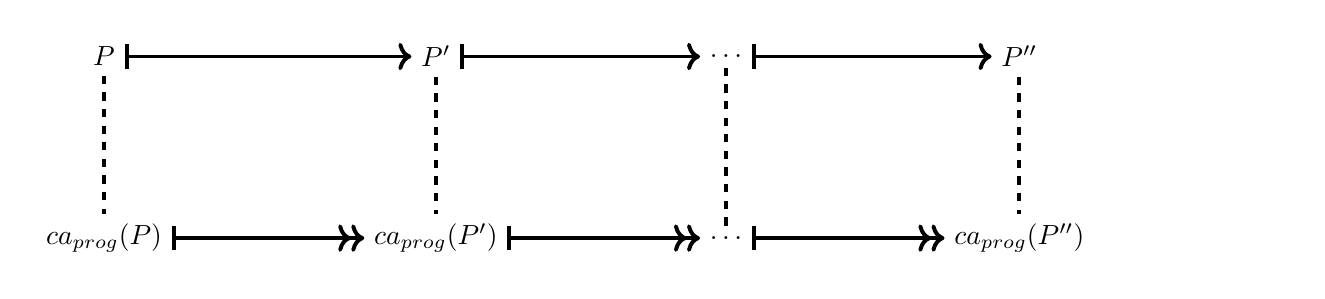
\begin{tikzpicture}[label/.style = {  }]
  \tikzset{every node/.style={anchor=center, text centered}} 
  \matrix (m)
    [
      matrix of math nodes,
      row sep    = 5em,
      column sep = 7em
    ]
    {
      P & P' & \dots & P'' & \\
      ca_{prog}(P) & ca_{prog}(P') & \dots & ca_{prog}(P'') \\
    };
  \foreach \i in {1, 2} {
    \path
      let \n1 = { int(\i+1) } in
        [line width=0.5mm ] (m-1-\i) edge [|->] node [above, label] {} (m-1-\n1)
        [line width=0.5mm ]  (m-2-\i) edge [|->>] node [below, label] {} (m-2-\n1);
  }
  \foreach \i in {1,...,3} {
    \path
      let \n1 = { int(\i+1) } in
          [line width=0.5mm] (m-1-\i) edge [dashed] node [left,  label] {} (m-2-\i);
  }
  \path [line width=0.5mm]  (m-1-3) edge [|->] node [left,  label] {} (m-1-4)
        [line width=0.5mm] (m-2-3) edge [|->>] node [left,  label] {} (m-2-4)
        [line width=0.5mm] (m-1-4) edge [dashed] node [left, label] {} (m-2-4);
\end{tikzpicture}
    \caption{Simulation relation visualization}
    \label{fig:sim_diagram}
\end{figure}

If we can show that $ca_{prog}$ is a simulation, then we know that $P$ and $ca_{prog}(P)$ take equivalent steps and therefore that $ca_{prog}$ preserves the semantics of the programs it transforms.

As a summary, our definitions so far are as follows:
\begin{table}
    \centering
    \begin{tabular}{ |c|p{6cm}|p{6cm}| } 
 \hline
 Symbol & Definition \\ 
 \hline
 $\step$& A single, standard, reduction step defined by the semantics. \\ 
 \trstep & The reflexive, transitive closure of $\step$ \\
 $ca_{prog}$ & $ca$ on programs. \\
 $ca_{ctx}$ & $ca$ on evaluations contexts. \\
 $ca_{sf}$ & $ca$ on store locations. \\
 $ca_{e}$ & $ca$ on expressions. \\ 
 \hline
\end{tabular}
    \caption{Definitions}
    \label{tab:defs}
\end{table}


Our proof is structured as follows:
\begin{enumerate}
    \item Show that our semantics is deterministic (Section \ref{sxn:det_sem}).
    \item Prove that $ca_{prog}$ is a simulation relation (Section \ref{sxn:sim}).
\end{enumerate}


\subsection{Deterministic Semantics}\label{sxn:det_sem}
An implicit assumption made by figure \ref{fig:sim_diagram} is that our programs only have one potential step to take. That is, that a program P will always step to the same P'. Another way of stating this is by saying that our semantics are \textit{deterministic}.

\begin{definition} Deterministic Relation

If a relation R is deterministic then,

$\forall a\ b_1\ b_2, a\ R\ b_1, a\ R\ b_2 => b_1 = b_2$.

\end{definition}

In the context of our semantics, we state this theorem as follows:

\begin{theorem}\label{thm:step_det}


\textbf{Single Step Deterministic}

$\forall P\ P_1\ P_2,\ P\ \step\ P_1,\ P\ \step\ P_2\ => P_1 = P_2$


\end{theorem}

To prove Theorem \ref{thm:step_det}, we will first show a property of all programs called the VSR property. This property states that P is either a \textbf{V}alue, \textbf{S}tuck, or \textbf{R}educible. In the context of our semantics, we say that that P is reducible if it can be decomposed into a context C and expression e such that $C[e]\ \step\ C'[e']$ for some $C'[e']$ on the right hand side of a semantic step. To show that our semantics are deterministic, we strengthen this property to require uniqueness of the evaluation context C that P decomposes into.

\begin{lemma}\label{lem:vsr} VSR Property for Programs

$\forall P,$ P is one of the three:
\begin{enumerate}
    \item $P = (store\ (sf\ \dots)\ v)$ --- Value
    \item $\lnot\ \exists P',\ P\ \step P'$ --- Stuck
    \item $\exists\ unique\ C, \ P = C[e], C[e]\ \step\ C'[e']$ --- Reducible
\end{enumerate}
\end{lemma}
\begin{proof} $\\$
By definition, P must be of the form $(store\ (sf\ \dots)\ e)$.

We can see that the VSR property holds for a program if it holds for the program's expression:

If $e$ is a value, then $P = (store\ (sf\ \dots)\ v)$.

If $P = (store\ (sf\ \dots)\ [e])$ has no applicable semantic steps to take, we say $e$ is stuck. Clearly in this case, $\lnot\ \exists P',\ P\ \step P'$

Finally, if $e = F[e']$ such that e' is a reducible expression, then $C[e] = C[F[e']]$ has a valid semantic step. We refer to this as $e$ being \textit{reducible}.

We proceed by induction on $e$.

If $e$ is a value, then we are done.

Otherwise, if e is not a value, consider the cases:

\textbf{Case 1: $e = (begin\ e_1\ e_2\ \dots)$}

We know by induction hypothesis that all $e_i$ in the body of the begin expression are either values, stuck, or reducible.

Consider when $e_2\ \dots$ is empty. Therefore, $e = (begin\ e_1)$. Hence, we can directly apply the \textbf{beginD} rule. Therefore, e is reducible, and the unique context is simply the store and an empty hole.

If $e_2\ \dots$ is not empty, then consider the case where $e_1$ is a value. Then, we can decompose $e$ into $F[v]$, where $F = (begin\ [\ ]_{*}\ e_2\ e_3\ \dots)$. The \textbf{promote} rule is applicable here, and there is no other decomposition we can perform on e. Therefore, this case falls under reducible. Next, consider when $e_1$ is stuck. Similar to the value case, the evaluation context for begin applies to e, but since $e_1$ is not a value, \textbf{promote} is not applicable. Therefore, we are stuck, since there is no applicable rule or further decomposition that would allow a step to be taken. Finally, consider the case where $e_1$ is reducible. Since $e_1$ is not a value, \textbf{promote} again cannot apply.  Then, we can decompose e into $F[e_1']$, where $F = (begin\ [\ ]\ e_2\ e_3\ \dots)$. Since \textbf{promote} and \textbf{beginD} are not applicable, F is the unique decomposition, with whichever reduction step $F[e_1']$ takes being the only applicable step.

\textbf{Case 2: $e = (if\ e_1\ e_2\ e_3)$}

If $e_1$ is a value, then either \textbf{ifT} or \textbf{ifF} are applicable, and $e$ is clearly reducible, with the unique context just being the store and an empty hole.

Otherwise, if $e_1$ is stuck and not a value, then $e$ is stuck. 

Similarly, if $e_1$ is reducible, then $e$ is reducible:

$e = F[e_1]$, where $F = (if\ [\ ]\ e_2\ e_3)$.

\textbf{Case 3: $e = (e_1\ e_2\ \dots)$}

Again, we know that all $e_i$ in the body of e are either values, stuck, or reducible.

Consider when all $e_i$ are values. Then, there can be various rules applied, depending on the specific value of each $e_i$: \textbf{cons, car, cdr, set-car!, set-cdr!, appN!, appN, app0} and all of the arithmetic rules are potentially applicable here. If none of these rules are applicable, then $e$ is stuck, since none of $e_i$ are further reducible.

If all of $e_i$ are stuck non-values, then $e$ can take the \textbf{mark} step and is therefore reducible (though it will be stuck immediately after). The same follows if all of $e_i$ are reducible non-values, except it will continue to take steps after.

Now, consider if $e_i$ are a mix of stuck, reducible, and value expressions. There are three possible cases here:

\begin{enumerate}
    \item $e$ can be decomposed into $F[e']$, where $F = (v\ \dots\ F_{\circ}\ v\ \dots)$.
    \item The \textbf{mark} rule is applicable.
    \item $e$ is stuck.
\end{enumerate}

We know this because \textbf{mark} is the only semantic rule applicable to $(e_1\ e_2\ \dots)$ expressions with non-value sub-expressions. However, due to the requirement of \textbf{mark} that $e_2\dots$ contains a non-value expression, it is never the case that \textbf{mark} can be applicable and $e$ can be decomposed using the $(v\ \dots\ F_{\circ}\ v\ \dots)$ evaluation context at the same time. If \textbf{mark} is not applicable, and a decomposition into the $(v\ \dots\ F_{\circ}\ v\ \dots)$ evaluation context is not possible, then $e$ is clearly stuck, since there are no other applicable semantic rules or possible evaluation context decompositions.

Therefore, consider the possibilities of $e'$ in the decomposition case. $e'$ cannot be a value, since then all of $e_i$ would be values, which contradicts our assumption. If $e'$ is reducible by some semantic step, then that is the semantic step that $e$ must take. Otherwise, if $e'$ is stuck, then $e$ is stuck, since all other $e_i$ are values.

In the \textbf{mark} and stuck cases, $e$ is clearly reducible and stuck respectively.


\textbf{Case 4: $e = (set!\ x\ e_1)$}

If $x$ is not in the store, e is clearly stuck, so we consider the case where $x$ is in the store.

By induction principle, $e_1$ must be a value, stuck, or reducible.

If $e_1$ is a value, the \textbf{set!} rule is applicable.

Otherwise, if not, $e$ is stuck if $e_1$ is, or reducible if $e_1$ is, with the $(set!\ x\ F_{\circ})$ evaluation context being the only possible decomposition, and therefore unique.

\textbf{Case 5: $e = (values\ v)$}

If $e$ is in a $[\ ]_{\circ}$ context, then \textbf{demote} is applicable, and $e$ is therefore reducible. Otherwise, it is stuck.

\textbf{Case 6: $e = x$}

If $x$ is in the store, then \textbf{var} is applicable, and $e$ is therefore reducible. Otherwise, $e$ is stuck.

By showing this property for all cases of P and e, we have proven it is true for all programs by induction principle.
\end{proof}

Since we have shown that if a program reduces, it does so by decomposing uniquely into an evaluation context and a reducible expression, Theorem \ref{thm:step_det} follows from Lemma \ref{lem:vsr}. That is, if $P = C[e]$, $P\ \step\ P_1$, and $P\ \step\ P_2$, then $P_1 = P_2 = C'[e']$ by Lemma \ref{lem:vsr}.

\subsection{$ca_{prog}$ is a simulation relation.\label{sxn:sim}}
In this section we show that the relation defined by the \textit{np-convert-assignments} pass is a simulation relation. First, we formally define our notion of simulation:

\begin{definition} \textbf{Simulation Relation}

If a relation R is a simulation, and $aRb$, then:

$a\ \step\ a' => \exists\ b', b$ \trstep\ $b', a'Rb'$
\end{definition}

That is, if $a$ and $b$ are related by a simulation relation, and $a\ \step\ a'$, then there must exist $b'$ such that $b$ \trstep\ $b'$ and that $a'$ is related to $b'$. Thus, to show that $ca$ is a simulation relation, we must show that if $P\ \step\ P'$, then there exists a ${P^{*}}$ such that $ca_{prog}(P)\ \trstep\ {P^{*}}, ca_{prog}(P') = {P^{*}}$.

Therefore, if we can show that for each possible single semantic step, that transforming the left hand side and then stepping a finite number of times always arrives at the transformation of the right hand side, then we have shown that $ca_{prog}$ is a simulation relation.

One thing to note is that since we are considering the decomposed programs that $\step$ operates on, we make implicit use of Lemma \ref{lem:trans_val} throughout our proof to relate these findings back to $ca_{prog}$.


\begin{theorem}\label{thm:step} \textbf{Step Theorem}


$P\ \step\ P' =>\\ \exists {P^{*}}\ such\ that\\ \ ca_{prog}(P)\ \trstep\ {P^{*}}\ and\\ \qquad ca_{prog}(P') = {P^{*}}$.

\end{theorem}
\begin{proof} By induction on the structure of P.

By Lemma \ref{lem:vsr}, P must be a value, be stuck, or be decomposible into a unique evaluation context C and a  expression e such that one of the semantic rules applies.

If P is a value or stuck, the theorem is trivial by contradiction.

Otherwise, P must be in the form of the left hand side of one of the semantic rules. Our proof follows by case analysis of the semantic rules.

The most interesting example comes from the rule \textbf{appN!}. This should make sense, since \textbf{appN!} corresponds to lambda applications that contain assignments, and $ca_{prog}$ removes all assignments. Indeed, we will confirm from the steps that correspond to \textbf{appN!} that assignments are removed.

First, we define some convenient notation:
\begin{table}[h]
    \centering
    \begin{tabular}{c}
         $\hat{P} = ca_{prog}(P)$  \\
         
        $\hat{C} = ca_{ctx}(C)$     \\

        $\hat{sf} = ca_{sf}(sf)$    \\

        $\hat{e} = ca_e(e)$     \\
    \end{tabular}
    \caption{Notation for various $ca$ functions}
    \label{tab:ca_notation}
\end{table}

Now, consider the semantic step \textbf{appN!}, taking $P$ to $P'$: 
\[
P = (store\ (sf \dots) F[((lambda\ (x)\ e)\ v)])\ \step 
\]
\[
P' = (store\ (sf \dots (p\ v)) F[(lambda\ ()\ \{x \xrightarrow{} p\}\ e)]) \quad (p\ fresh,\ x\ assigned\ to\ in\ e)
\]

$P$ transforms to $\hat{P}$:
\[
\hat{P} = (store\ (\hat{sf} \dots) \hat{F}[((lambda\ (t)\ ((lambda\ (x)\ \hat{e})(cons\ t\ null))\ \hat{v}))]) \quad (t\ fresh)
\]

$P'$ transforms to $\hat{P'}$:
\[
\hat{P'} = (store\ (\hat{sf} \dots (pp\ (cons\ \hat{v}\ null)) \hat{F}[(lambda\ ()\ \{x \xrightarrow{} pp\}\ \hat{e})])
\]

If $ca$ is a simulation, $\hat{P}$ must take a finite amount of steps and arrive at a $P^{*}$ such that $P^{*} = \hat{P'}$.

We propose that $\hat{P}$ will take 5 steps to get to $P^{*}$.
\begin{enumerate}
    \item We first apply the \textbf{appN} rule to $\hat{P}$, since t is fresh.
    \[
    (store\ (\hat{sf} \dots) \hat{F}[((lambda\ (t)\ ((lambda\ (x)\  \hat{e})(cons\ t\ null))\ \hat{v}))])\ \step
    \]
    \[
    (store\ (\hat{sf} \dots) \hat{F}[((lambda\ ()\ ((lambda\ (x)\  \hat{e})(cons\ \hat{v}\ null))))])
    \]
    \item Then, we apply \textbf{app0}.
    \[
    (store\ (\hat{sf} \dots) \hat{F}[((lambda\ ()\ ((lambda\ (x)\  \hat{e})(cons\ \hat{v}\ null))))])\ \step
    \]
    \[
    (store\ (\hat{sf} \dots) \hat{F}[((begin\ ((lambda\ (x)\  \hat{e})(cons\ \hat{v}\ null))))])
    \]
    \item Now, we apply \textbf{beginD}.
    \[
    (store\ (\hat{sf} \dots) \hat{F}[((begin\ ((lambda\ (x)\  \hat{e})(cons\ \hat{v}\ null))))])\ \step
    \]
    \[
    (store\ (\hat{sf} \dots) \hat{F}[((lambda\ (x)\  \hat{e})(cons\ \hat{v}\ null))])
    \]
    \item At this point, to apply the \textbf{cons} rule, we must first decompose our program into an evaluation context and a reducible expression. We do so as follows:
    \[
    (store\ (\hat{sf} \dots) \hat{F}[((lambda\ (x)\  \hat{e})(cons\ \hat{v}\ null))]) = 
    \]
    \[
    (store\ (\hat{sf} \dots) \hat{F_{+}}[(cons\ \hat{v}\ null)])
    \]
    where $\hat{F_{+}} = \hat{F}[((lambda\ (x)\ \hat{e})[\ ])]$.
    
    We can then reduce using the \textbf{cons} rule:
    \[
    (store\ (\hat{sf} \dots) \hat{F_{+}}[(cons\ \hat{v}\ null)])\ \step
    \]
    \[
    (store\ (\hat{sf} \dots (pp\ (cons\ \hat{v}\ null))) \hat{F_{+}}[pp])
    \]
    And expand our context:
    \[
    (store\ (\hat{sf} \dots (pp\ (cons\ \hat{v}\ null))) \hat{F_{+}}[pp]) = 
    \]
    \[
    (store\ (\hat{sf} \dots (pp\ (cons\ \hat{v}\ null)))\hat{F}[((lambda\ (x)\ \hat{e})\ pp)]
    \]
    
    
    \item Finally, we can apply \textbf{appN} again, since pp is fresh.
    \[
    (store\ (\hat{sf} \dots (pp\ (cons\ \hat{v}\ null))) \hat{F}[((lambda\ (x)\  \hat{e})\ pp)])\ \step
    \]
    \[
    (store\ (\hat{sf} \dots (pp\ (cons\ \hat{v}\ null))) \hat{F}[(lambda\ ()\  \{x \xrightarrow{} pp\}\ \hat{e})])
    \]
\end{enumerate}

Comparing this result to $\hat{P'}$, we can see they are the same. Therefore, if $P$ takes step \textbf{appN!}, $\hat{P}$ takes the steps \textbf{appN, app0, beginD, cons, appN} in order to arrive at a $P^{*}$ that satisfies our simulation definition. Figure \ref{fig:appn!_steps} visualizes this relationship.

\begin{figure}[h]
    \centering
    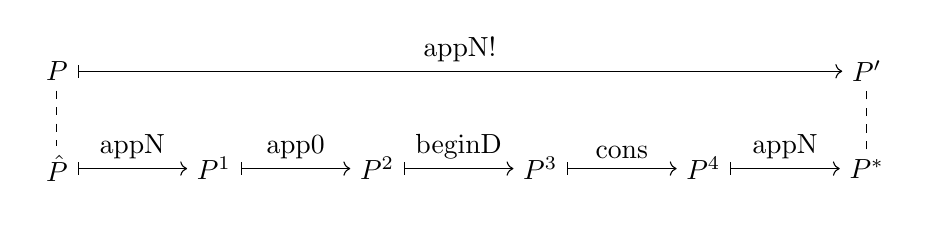
\begin{tikzpicture}[label/.style = {  }]
  \tikzset{every node/.style={anchor=center, text centered}} 
  \matrix (m)
    [
      matrix of math nodes,
      row sep    = 2em,
      column sep = 4em
    ]
    {
      P & & & & & P' \\
      \hat{P} & P^{1} & P^{2} & P^{3} & P^{4} & P^{*} \\
    };
    \path
        (m-2-1) edge [|->] node [above, label] {appN} (m-2-2)
        (m-2-2) edge [|->] node [above, label] {app0} (m-2-3)
        (m-2-3) edge [|->] node [above, label] {beginD} (m-2-4)
        (m-2-4) edge [|->] node [above, label] {cons} (m-2-5)
        (m-2-5) edge [|->] node [above, label] {appN} (m-2-6)
        (m-2-6) edge [dashed] node [] {} (m-1-6)
        (m-1-1) edge [dashed] node [] {} (m-2-1)
        (m-1-1) edge [|->] node [above, label] {appN!} (m-1-6);
\end{tikzpicture}
    \caption{Simulation of \textbf{appN!}}
    \label{fig:appn!_steps}
\end{figure}

It turns out this is the only case where more than one equivalent step is taken. In the cases of \textbf{var} and \textbf{set}, $\hat{P}$ takes a \textit{different} step, but still only takes one:

\begin{figure}[h]
\centering
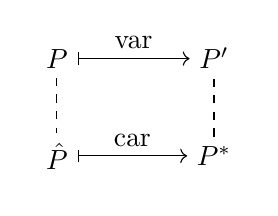
\begin{tikzpicture}[label/.style = {  }]
  \tikzset{every node/.style={anchor=center, text centered}} 
  \matrix (m)
    [
      matrix of math nodes,
      row sep    = 2em,
      column sep = 4em
    ]
    {
      P & P' \\
      \hat{P} & P^{*} \\
    };
    \path
        (m-2-1) edge [|->] node [above, label] {car} (m-2-2)
        (m-2-2) edge [dashed] node [] {} (m-1-2)
        (m-1-1) edge [dashed] node [] {} (m-2-1)
        (m-1-1) edge [|->] node [above, label] {var} (m-1-2);
\end{tikzpicture}
\qquad
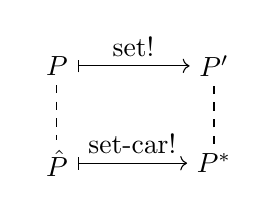
\begin{tikzpicture}[label/.style = {  }]
  \tikzset{every node/.style={anchor=center, text centered}} 
  \matrix (m)
    [
      matrix of math nodes,
      row sep    = 2em,
      column sep = 4em
    ]
    {
      P & P' \\
      \hat{P} & P^{*} \\
    };
    \path
        (m-2-1) edge [|->] node [above, label] {set-car!} (m-2-2)
        (m-2-2) edge [dashed] node [] {} (m-1-2)
        (m-1-1) edge [dashed] node [] {} (m-2-1)
        (m-1-1) edge [|->] node [above, label] {set!} (m-1-2);
\end{tikzpicture}
    \caption{Simulation of \textbf{var} and \textbf{set!}}
    \label{fig:varcar_steps}
\end{figure}

%show var, set 

For all other steps, since the $ca$ functions don't affect the LHS in a meaningful way, $ca_{prog}(P)$ takes the same step that $P$ does.

This relationship is shown in Figure \ref{fig:sem_steps}:

\begin{figure}[h]
    \centering
    \begin{tabular}{c|c}
     Semantic Step & Steps for $\hat{P}$ to reach ${P^{*}}$ \\
     \hline
     appN! & appN, app0, beginD, cons, appN \\
     var & car \\
     set! & set-car! \\
     All other steps & Same step \\
    \end{tabular}
    \caption{Equivalent semantic steps before and after \caname.}
    \label{fig:sem_steps}
\end{figure}

Therefore, we have shown that $ca_{prog}$ is a simulation relation. 
\end{proof}

\subsection{\caname\ is semantic preserving}\label{sxn:ca_sem_pres}

Now that we know that $ca_{prog}$ is a simulation relation, we can see that it preserves semantics. 

For example, if $P$ \trstep $P'$, then by Theorems \ref{thm:step_det} \& \ref{thm:step} and induction on the number of steps taken by $P$, we can easily see that $ca_{prog}(P)$ \trstep $\ ca_{prog}(P')$. Therefore, if $P$ gets stuck, gets to a value, or continues infinitely, $ca_{prog}(P)$ will take equivalent steps and get to the transformed version of the stuck expression, of the value expression, or of an arbitrary expression in the infinite sequence.
\chapter{Validation Frameworks\label{chap:valid}}
In chapter \ref{chap:proof}, we give a "paper" proof of the correctness of the \textit{convert-assignments} pass. However, we still need to verify that our proof is correct. While we have carefully checked our assumptions and the overall chain of logic of our paper proof, it is always possible to make mistakes or overlook logical flaws when manually reviewing. Fortunately, as covered in section \ref{background}, there are powerful proof assistants available that can aid in \textit{mechanizing} proofs such as ours. In addition, we have the luxury of having access to an existing implementation of the R6RS semantics that allows us to test examples to ensure that $ca_{prog}$ satisfies the requirements of being a simulation relation.

Our initial goal for this project was to provide a full formal mechanization of our proof using the Coq proof assistant. However, the advanced detail required made a complete mechanization out of the scope of this thesis work. Still, we successfully implemented a portion of the R6RS semantics as well as a model of the pass itself in Coq. We will show later in the section some details of the implementation as well as how it could be extended to complete formalization of our proof, and therefore prove to a high degree of certainty the correctness of the \textit{convert-assignments} pass.

Although we were not able to completely formalize the proof in Coq, we wanted to be able to at least test some examples and have empirical evidence of the validity of our proof. To do so, we provide a testing framework based on an existing implementation of the R6RS semantics. We use this testing framework to show that the \textit{convert-assignments} pass is in fact a simulation relation for a variety of Scheme programs. This implementation and its 

\section{Coq Framework}
\subsection{Overview and Functionality}
We provide an implementation of a subset of the R6RS formal semantics as well as a model of the \caname\ pass. In addition, we prove some properties of the semantics, such as the property that substituting a fresh variable in an expression returns that same expression. Whereas in our paper proof, we may assume that this is true, Coq requires you to explicitly prove the validity of seemingly obvious properties such as this one. For example, in our proof of the VSR property for programs (Lemma \ref{lem:vsr}), at one point we need to show that a program not in the form of any semantic step is stuck. In our paper proof, we do not provide much detail here, as it fairly obvious that a program that does not match a semantic step has no applicable semantic steps. However, in Coq, we would need to explicitly show that if such a program could step, that it would lead to a logical inconsistency. In addition, we would have to show this for all such trivially stuck programs. While we can abstract properties like this out to seperate lemmas, mechanization of a proof like ours requires an amount of detail that is simply not needed for even a very strong paper proof. Therefore, while we have a formal model of our subset of the R6RS semantics and some properties of the semantics verified, there are many more minor properties need to be proven to be able to formally verify the overall correctness of the pass.

In terms of present functionality, our implementation does provide a way of manually applying semantic steps, and we show some simple examples by proving, for example, that $(car\ (cons\ v_1\ v_2)) = v_2$ for all $v_1, v_2$. Again, while this is quite a trivial proof on paper, Coq requires explicit evidence of its truth, which we show by stepping through the appropriate semantic steps in a systematic way.

Finally, implementing the semantics and pass in Coq required some specific nuance unique to Coq and the context of programming language metatheory proofs. We discuss these implementation details in section \ref{sxn:impl}.
\subsection{Implementation Details\label{sxn:impl}}
Our implementation of an operational semantics for Scheme programs follows closely from the implementation included with R6RS --- however, encoding this semantics in Coq presents challenges unique to the intricacies of the Coq language.
\subsubsection{Capture-Free Substitution}
Historically, handling variable bindings has been a major hurdle in proofs about programming language metatheory \cite{}. Specifically, the issue of implementing a substitution operation while avoiding unwanted capture of variables is extremely important, but can be difficult to accomplish in mechanized proofs. If a semantic model uses named variables, the proof authors must now reason about all possible names in every relevant lemma that they prove. Since programming languages tend to allow developers close to free reign with defining names for variables, trying to reason about all possible names in expressions quickly becomes intractable. 

In paper proofs, this problem is dealt with by freely applying $\alpha$-conversion if capture would occur, or simply by using the same variables and assuming that no capture occurs. This means that in paper proofs, and in our minds, we tend to implicitly work with $\alpha$-equivalence classes of expressions rather than directly with expressions themselves. For example, we naturally consider expressions ($\lambda (x) x$) and ($\lambda (y) y$) as equivalent.

To remedy the problem of reasoning over all possible names, and more closely emulate our intuition and the typical form of reasoning seen in paper proofs, we use the locally nameless style of variable bindings in our formal model. This style uses de Bruijn indices for bound variables (hence \textit{locally nameless}), and names for free variables. Hence, lambda expressions within this system are syntactically equivalent if they are in the same $\alpha$-equivalence class.

Some examples of de Bruijn indexed expressions:

($\lambda$ (bvar 0)) is the identity function

($\lambda$ ($\lambda$ (+ (bvar 0) (bvar 1)))) is an addition function.

Notice that lambda expressions have no formal arguments. This is because bound variables are "nameless" in this system. Instead, the index of a bound variable refers to the level of abstraction. So (bvar 0) refers to a variable bound by the immediately surrounding abstraction. Whereas (bvar 1) refers to a variable bound by an abstraction surrounding the immediate abstraction.

\subsubsection{Cofinite Quantification}
Cofinite quantification is a small stylistic change to the normal way of defining substitution that allows us to have a slightly more powerful induction principle when dealing with fresh variable substitution.

Traditionally, a fresh variable is generated by simply picking (existential quantification) a single variable not in the set of free variables of the expression it is being substituted in. In the cofinite quantification style, we use universal rather than existential quantification to reason about all fresh variables instead of a single one. That is, our defintion of freshness generalizes to say all variables x not in some set L are fresh. In our definition for freshness of a variable with respect to an expression, we say the set L is the set of free variables in the expression. Because of this, where we would reason about a single fresh variable, we instead are reasoning about the set of all fresh variables, which can help with showing that a variable that is fresh in an expression is also fresh in its sub-expressions.

\subsubsection{Step-Indexed Evaluation}
To reason about non-terminating programs while still satisfying the requirement that all Coq functions terminate, we use step indexing on many of our functions. This means that our functions are given an index to keep track of how many "steps" they have taken, with a limit that causes termination after the index exceeds it. This ensures that all of our functions are terminating, while being flexible enough to account for large programs For functions dealing with nested sub-expressions, our step index usually refers to recursion depth rather than actual steps taken, so very large terms can be handled without necessarily setting a large step limit.
\section{Racket Framework}
\subsection{Overview and Functionality}
While our Coq framework approaches validation of our proof from the perspective of static analysis, our Racket framework instead provides a more "dynamic" means of checking validity of our proof against specific examples. Given a valid program in our subset of Scheme, our Racket framework uses an existing implementation of the R6RS formal semantics to perform a semantic step on the program. Then, it executes $ca_{prog}$ on the original program and verifies that stepping a finite number of times (in our case 5) contains the result from the single semantic step. 
\subsection{Implementation Details}
\subsubsection{Extensibility}
Because we are using the full R6RS semantics here, we can easily extend this framework to test examples outside of the scope of our original proof. All that needs to be done to add new kinds of expressions to the framework is extending the framework's implementation of $ca_{prog}$ to appropriately recurse on these new expression's sub-expressions. While this is not a substitute for a formal proof, one can reasonably assure themselves that our proof technique holds over a set of examples that include such new expressions. By constructing the framework in this way, we continue the pattern of high extensiblity in our reasoning.
\subsubsection{Evaluation Order}
As mentioned in section \ref{sxn:excluded}, we assume a left-to-right evaluation order in our proof. However, as we also mention, the R6RS semantics provides a way for implementations to specify the evaluation order by modifying the \textbf{mark} semantic rule. In this framework, we are of course relying on the un-modified \textbf{mark} rule, since we are directly applying the formal R6RS semantics. However, we circumvent this by simply choosing the path that corresponds to a left-to-right evaluation in all cases. A possible extension to this framework would be to consider all evaluation orders when testing an example for adherence to our proof technique. However, since we do not prove this in our paper proof, we kept the assumption of left-to-right evaluation for this framework.

\subsubsection{Testing Framework}
As previously mentioned, the purpose of this framework is to give a means of testing the validity of our proof by simulation approach. An example of this testing is shown by figure \ref{fig:rkt_sim_example}. It should be noted that we do not perform this validation by manual examination. 

\begin{figure}
    \centering
    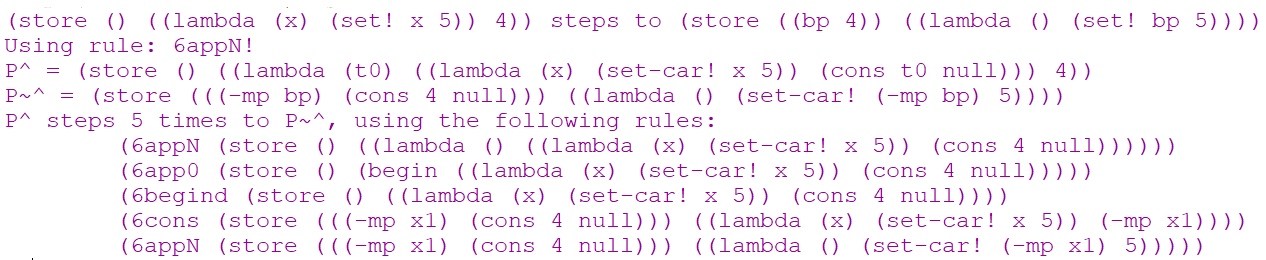
\includegraphics[ width=\textwidth]{figures/sim_example.PNG}
    \caption{Example of a Racket framework test case}
    \label{fig:rkt_sim_example}
\end{figure}

Figure \ref{fig:rkt_sim_example} is a text-based visualization of the process that our testing framework uses to validate our proof approach. In the full version of our test, we step until a limit is reached or no further steps are applicable and test the simulation relation for each step.

One very important detail of this framework can also be observed in figure \ref{fig:rkt_sim_example} --- that the terms we expect to match are not syntactically equivalent, but instead equal over $\alpha$-equivalence. To counteract this, in our test suites, we first normalize programs such that they are syntactically equal to all programs in their $\alpha$-equivalence class before comparing them. That way, we get positive results for comparing programs that are entirely the same except for a difference in naming. However, this also means that implicit shadowing or freshness of variables that have the same name is not allowed in this framework. Indeed, this makes it so that this framework does not typically mesh well with examples that include recursion, such as the Y-combinator.
\chapter{Conclusions and Future Work}
In this chapter, we conclude and summarize the project, reflect on our process of proof and in building our validation frameworks, and discuss future work on this project.

\section{Reflections}
The original intent of this work was to provide a full mechanization of the proof in Coq. To that end, some of the features removed were done so with the motivation of simplifying the Coq formalization. As we discuss in section \ref{sxn:coq_overview}, Coq requires a large amount of detail and specific proof of things that are seemingly given or obvious in a paper proof. For example, we prove in our framework that substitution of a fresh variable is the identity for the \textit{locally nameless} Scheme representation in our Coq framework, something that we take as given in our paper proof.

As our project's scope shifted to no longer target a full mechanization, some features were added back in to our model, but a project started with the intention of a paper proof only could have likely included the entire R6RS semantics, as the features we excluded are largely unaffected by $ca_{prog}$. While complicated features like quote would have added some complexity to the proof, the \caname\ pass does not modify quoted expressions. Therefore, the only additional complexity would be altering our various definitions to include, for example, additional 

Another feature, exceptions, may have actually aided our proof by giving an even stronger definition for \textit{stuck} programs. However, it is clear to see that \caname\ would behave no differently with this change, so its exclusion presents no threat to the overall validity of our claim of correctness.

\section{Future Work}
There are a few paths for potential future work on this project. The first would be extending the paper proof in one of two ways: extending the language we prove over, and/or proving correctness of another pass 

The second future work would be to continue the original scope of this project in fully mechanizing the current proof. This work would entail proving various lemmas to definitively prove Theorems \ref{thm:step_det} and \ref{thm:step} inside of our Coq framework. While our framework provides definitions for the syntax and semantics of our R6RS subset and some of the auxiliary lemmas, extending it to fully mechanize our proof would likely take some fine-tuning of the definitions, or more specific definitions of, for example, well-formed expressions, which we assume extensively throughout our paper proof.

\section{Summary and Closing}
In this work, we detailed the proof of correctness of our representation of the \caname\ pass, $ca_{prog}$. Most of our proof follows by induction on the structure of our programs and expressions, with extensive case analysis on programs formed such that a semantic step is applicable to them. We also provide frameworks in Coq and Racket for validation of our proof through computer-checked proof and testing of specific examples respectively. While we consider a subset of the R6RS semantics in all of our proofs, each has the possibility of extension to include a more complete version, though this would likely be quite difficult in the case of the Coq framework. Overall, this work provides a reasonably trustworthy proof of correctness of the \caname\ pass of the Chez Scheme compiler.

\nocite{*}
\bibliography{bibliography}

% Indents Appendix in Table of Contents
\makeatletter
\addtocontents{toc}{\let\protect\l@chapter\protect\l@section}
\makeatother

% Hack to make Appendices to appear in Table of Contents
\addtocontents{toc}{%
   \noindent APPENDICES
}
\begin{appendices}
\input{appendix-outline}
\end{appendices}

\end{document}
